%%% Local Variables:
%%% mode: latex
%%% TeX-master: "../doc"
%%% coding: utf-8
%%% End:
% !TEX TS-program = pdflatexmk
% !TEX encoding = UTF-8 Unicode
% !TEX root = ../doc.tex

3D-Visualisierungen werden in vielen Branchen verwendet. \e{Virtual Reality}, CAD-Programme oder Computerspiele sind einige bekannte Anwendungsgebiete. Dank leistungsfähigeren Geräten sind realistischere Visualisierungen möglich.

Anwendungen können auf spezifische Hardware, wie zum Beispiel die Spielkonsole PlayStation, ausgerichtet sein. Es gibt Unterschiede zwischen den Konsolen, grundsätzlich sind die Variationen der Leistungsfähigkeit innerhalb einer Konsolengeneration klein. In anderen Anwendungsfällen kann eine Applikation sogar für nur eine spezifische Hardware entwickelt werden. Dies erlaubt es, eine Applikation auf die Anforderungen dieser Hardware zuzuschneiden. Der primäre Nachteil ist die Zugänglichkeit der Software, da spezifische Hardware notwendig ist. So ist es einerseits aufwändig, die Hardware zu beschaffen, andererseits aber auch eine Kostenfrage. Für gewisse Anwendungsgebiete ist dies jedoch ein sekundäres Problem.

Für hardwareunabhängige Anwendungen eignet sich die Web-Plattform hervorragend.
Immer mehr Benutzer haben Zugang zu einem Desktop, Tablet, Mobiltelefon oder zu einem anderen Gerät, welches Zugang zum Internet bietet \cite{peopleWithInternetAccess}.
Somit ermöglicht die Web-Plattform, Anwendungen mit weniger Aufwand einem grossen Zielpublikum zugänglich zu machen.
Seit einigen Jahren ist es auch möglich, 3D-Visualisierungen im Web zu realisieren.

\section{Kontext}
In dieser Arbeit wird der Fokus auf die Web-Plattform gelegt. Die Grundlagen sind jedoch auch in anderen Entwicklungsumgebungen zutreffend.
Für die Vereinfachung wird im Folgenden der Begriff Web für die Plattform von verschiedenen Web-Technologien genutzt. Dies beinhaltet insbesondere vom \e{World Wide Web Consortium}, kurz W3C, veröffentlichte Standards.

\section{Ausgangslage}
Dank der Rechenleistung auf modernen Geräten ist es möglich, anspruchsvolle 3D-Visualisierungen in Echtzeit auf diversen Geräten zu implementieren. Da diese Applikationen rechenintensiv sind und gerade mobile Geräte in ihrer Rechenleistung beschränkt sind, ist Performanzoptimierung im 3D-Rendering unabdinglich. Insbesondere die Komplexität der Modelle hat einen signifikanten Einfluss auf die Leistung.
Eine Möglichkeit zur Optimierung ist das Anzeigen von vereinfachten Modellen ab bestimmten Distanzen zum Betrachter. So kann zum Beispiel ein Modell in grosser Distanz vereinfacht dargestellt werden (Abbildung \ref{fig:lodComparisonSimplified}), solange bei genauer Betrachtung mehr Details sichtbar werden (Abbildung \ref{fig:lodComparisonOriginal}).

\begin{figure}[H]
  \centering
  \begin{subfigure}{.4\textwidth}
    \centering
    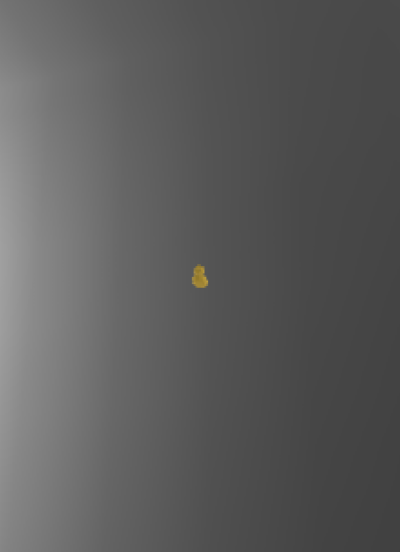
\includegraphics[width=.8\linewidth]{resultate/simplified-distance.png}
    \caption{vereinfachtes Modell entfernt}
    \label{fig:lodComparisonSimplified}
  \end{subfigure}
  \begin{subfigure}{.4\textwidth}
    \centering
    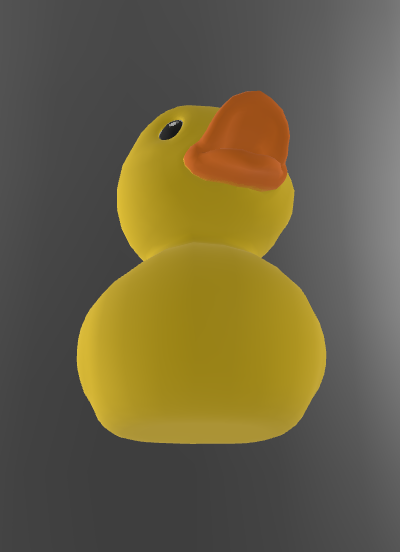
\includegraphics[width=.8\linewidth]{resultate/lod-original.png}
    \caption{Originalmodell nah}
    \label{fig:lodComparisonOriginal}
  \end{subfigure}
  \caption{Vergleich vereinfachtes Modell (entfernt) Originalmodell (nah)}
\end{figure}

In diversen \fglspl{Rendering Engine}{Programm, das zuständig für die Darstellung von 3D-Grafiken ist} gibt es deshalb Optionen für das Verwenden von sogenannten Level Of Details (\e{LOD}) Artefakten.
Für \fgls{Game Engines}{Framework für Computerspiele, das für den Spielverlauf und dessen Darstellung verantwortlich ist} wie \e{Unreal Engine} oder \e{Unity} gibt es bewährte Tools, um den Einsatz von \e{LOD}-Artefakten zu vereinfachen. Zurzeit gibt es in der Web-Entwicklung keine weitverbreitete Möglichkeit für das Generieren von solchen Artefakten.

\subsection{3D-Rendering im Web}

Als Basis für 3D-Visualisierungen im Web dient meist das von der \e{Khronos Group} entwickelte \e{WebGL}, das von allen modernen Browsern unterstützt wird. \e{WebGL} ist eine \e{Low Level JavaScript API} für 3D-Visualisierungen \cite{webGl1Spec}.
Als Alternative wird zurzeit ein weiterer Standard entwickelt: \e{WebGPU}. Dieser ist aktuell noch in Entwicklung und wird deshalb nicht weiter berücksichtigt, auch wenn ein grosses Potenzial vorhanden ist \cite{webGPUCharter}.

Die Unabhängigkeit der Hardware bedeutet, dass Optimierung der Performanz in Web-Anwendungen notwendig ist, um allen Benutzern ein optimales Erlebnis zu ermöglichen.
Im Vergleich zu fixen Hardwareanwendungen ist es realistisch, dass eine Web-Anwendung sowohl auf einem leistungsfähigen Desktop Computer als auch auf einem günstigen Mobilgerät verwendet wird.

\pagebreak

Zudem ist \e{WebGL} eine junge Technologie und wurde erst 2011 veröffentlicht \cite{webGl1Spec} – verglichen mit dem initialen Veröffentlichungsdatum von \fgls{OpenGL}{Spezifikation einer Programmierschnittstelle zur Entwicklung von 2D- und 3D-Grafikanwendungen} welches im Jahre 1992 publiziert wurde \cite{openGlSpec}.
Nicht nur das Alter, sondern auch die Natur der Web-Plattform hat dazu beigetragen, dass \e{WebGL} ein langsames Wachstum verspürt hat. Um einen Webstandard wie \e{WebGL} einsetzen zu können, müssen alle grossen Browser die Spezifikation implementieren. Ansonsten kann der grosse Vorteil des Webs – einfache Verteilung an alle Benutzer – nicht in vollem Umfang genutzt werden. So hat zum Beispiel der Internet Explorer 10 keinen Support und es wurde deshalb erstmals Ende 2013 möglich, im Internet Explorer 11 3D-Anwendungen für ein breites Publikum zu entwickeln.

\subsection{JavaScript Bibliotheken}
Um die Arbeit mit \e{WebGL} zu vereinfachen, gibt es verschiedene \e{High Level JavaScript} Bibliotheken. Die bekanntesten werden hier kurz erwähnt. Als Indikator für die Popularität wurden die wöchentlichen Downloads auf \fgls{npm}{Node Package Manager, Datenbank von JavaScript Paketen und Paketmanager.} verwendet. Wichtig ist, dass dies alleine keinen verlässlichen Indikator darstellt – für eine kurze Übersicht jedoch ausreichend geeignet ist.

\paragraph{Three.js}
\e{Three.js} ist die wohl weitverbreiteste Bibliothek für 3D-Rendering im Web \cite{threeNpmPackage}.
Die Community von \e{Three.js} ist aktiv und das offene Produkt wird kontinuierlich weiterentwickelt. Insbesondere die Erweiterungen \cite{threeFiberGithub} für \e{React}, eine populäre Bibliothek für die Entwicklung von Frontend Applikationen \cite{reactNpmPackage}, zeigen den Innovationsdrang.
Die Hauptvorteile liegen in der weiten Verbreitung, dem grossen Fokus auf Performanz und einem soliden Set an Basisfeatures. Elemente wie eine \e{Physics Engine} fehlen jedoch und müssen vom Entwickler integriert werden. Zudem setzt \e{Three.js} nicht auf \fGls{Semantic Versioning}{Konvention für Veröffentlichung von Software Paketen, siehe: semver.org \cite{semanticVersioning}}, was bedeutet, dass jede neue Version potenziell nicht rückwärtskompatible Änderungen beinhalten kann.

\paragraph{Babylon.js}
Eine weitere offene Bibliothek ist \e{Babylon.js}, welche die Entwicklung von 3D-Applikationen vereinfacht. Sie zeichnet sich vor allem durch einen grossen Funktionsumfang aus \cite{babylonjsNpmPackage}. So verfügt sie zum Beispiel über integrierte Erweiterungen für verschiedene \e{Physics Engines} und erleichtert somit den Einsatz von anspruchsvollen Features. Ausserdem setzt es auf \e{Semantic Versioning}.
Im Vergleich zu \e{Three.js} verfügt \e{Babylon.js} über eine kleine Community. Aufgrund dessen werden Erweiterungen für populäre Bibliotheken tendenziell weniger aktiv entwickelt.

\paragraph{PlayCanvas}
\e{PlayCanvas} ist eine offene 3D-Engine, welche primär für das Web entwickelt wurde. Als Erweiterung wird zudem ein proprietärer \e{Cloud Service} angeboten \cite{playcanvasNpmPackage}. Die Community ist – im Vergleich zur direkten Konkurrenz, wie zum Beispiel \e{Three.js} – klein. \e{PlayCanvas} verfolgt jedoch einen anderen Ansatz und liefert zum Beispiel eine standardmässige Integration für eine \e{Physics Engine}.

\paragraph{Unity}
\e{Unity}, welches vor allem für die Entwicklung von Mobile Applikationen bekannt ist, bietet seit längerer Zeit die Möglichkeit Projekte für das Web zu exportieren \cite{unityWeb}.
\e{Unity} bietet zwar den \e{Sourcecode} für Teile der \e{Engine} offen zur Verfügung, die Lizenz verbietet es jedoch den Code weiterzuverwenden \cite{unityOpenSource}.
Zudem bietet \e{Unity} keine zu \e{Three.js}, \e{Babylon.js} oder \e{PlayCanvas} vergleichbare Integration für die Web-Entwicklung an. \e{Unity} Projekte müssen direkt im \e{Unity Editor} entwickelt werden. Dies erschwert den Einsatz von \e{Best-Practices}, deshalb wird  \e{Unity} in dieser Arbeit nicht weiter berücksichtigt.

\subsection{Stand der Technik}

In anderen Umgebungen gibt es bereits umfangreiche \e{LOD}-Systeme für komplexe Anwendungsgebiete. Auf diese wird in der Sektion \autoref{chap:existingSolutions} detaillierter eingegangen.
Die erläuterten Bibliotheken bieten Funktionen für das Laden von \e{LOD}-Artefakten. Teilweise gibt es die Möglichkeit, Vereinfachungen im Browser zu generieren. Das Generieren von \e{LOD}-Artefakten zur Laufzeit ist jedoch für Web-Applikationen nicht geeignet, da dies signifikante Auswirkungen auf das Laufzeitverhalten hat und insbesondere auf schwächeren Geräten die Applikation zusätzlich verlangsamt.
So dauert das Optimieren eines komplexen Modells, wie zum Beispiel bei \e{Babylon.js} demonstriert, auch auf rechnungsstarken Geräten mehrere Sekunden \cite{babylonAutoLod}. \e{Three.js} verfügt über eine vergleichbare Möglichkeit, welche dieselben Limitationen aufweist \cite{threeSimplifyModifier}. Möchte man die Artefakte vorzeitig generieren, so ist es notwendig, diese Schritte manuell durchzuführen. Bei Modellanpassungen entsteht somit ein wiederkehrender manueller Aufwand. Ein Tool für die Konfiguration der Artefakte, wie dies bei \e{Unreal} oder \e{Unity} der Fall ist, steht nicht zur Verfügung.

Des Weiteren sind die Systeme nicht untereinander kompatibel. So kann das System zur Modellgenerierung von \e{Babylon.js} nicht in \e{Three.js} verwendet werden, obwohl die Problemstellung dies erlaubt. Folglich divergieren die Systeme und Weiterentwicklungen müssen für jedes System neu implementiert werden.

\pagebreak

\section{Zielsetzung}
Das Ziel der Arbeit ist es, ein Tool zu entwickeln, das den Umgang mit \e{LOD}-Artefakten im Web vereinfacht. Hierfür muss ein Algorithmus entwickelt werden, der es erlaubt, Modelle signifikant zu vereinfachen, ohne die grobe geometrische Form zu verlieren. Im Anschluss muss das Tool zur Verfügung gestellt werden, sodass es in der Praxis eingesetzt werden kann. Hierbei ist es wichtig, dass die Artefakte nicht innerhalb des Browsers generiert werden. Zudem soll der Einsatz des Tools einen möglichst geringen Zusatzaufwand bedeuten und für ein breites Spektrum an Modellen angewendet werden können. Ersteres wird dadurch ermöglicht, in dem ein Konfigurationstool bereitgestellt wird, mit dem man Konfigurationseinstellungen für die generierten Modelle vornehmen kann. Des Weiteren soll das Tool soweit erweiterbar sein, dass es für verschiedene Bibliotheken eingesetzt werden kann, ohne den Kern neu entwickeln zu müssen. Zudem muss der Beleg erbracht werden, dass das Laufzeitverhalten der Applikation mit \e{LOD}-Artfakten verbessert werden kann. Hierfür muss ein geeignetes Werkzeug zur Messung der wichtigsten Faktoren der Laufzeit definiert werden.
